


\begin{frame}{Pointsystem ved biotopplantiltag}

\begin{columns}[T] % T = top-aligned

\begin{column}{0.48\textwidth}
\textbf{Regler ved vegetationsstriber i marken:}
\begin{itemize}
    \item Biotopplaner inddeles i 3 typer (1-, 3- og 5-årige)
    \item 1-årige biotopplaner skal opfylde kravene på en samlet pointsum på minimum 100
    \item Min 3m bred
    \item Min 40m til kanten af det dyrkede areal
    \item Må ikke gødskes eller sprøjtes.
    \item Summen af point for tiltagene x 100 ha. / biotopplanejendommens areal i ha.
\end{itemize}
\end{column}

\begin{column}{0.4\textwidth}
    % Vælg én af disse – de ser godt ud i præsentation
    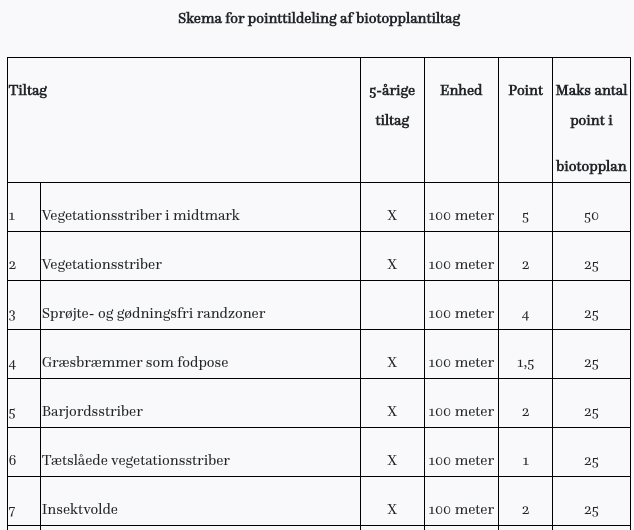
\includegraphics[width=\textwidth]{Billeder/Vildtforvaltning/biotopplantiltag/pointsystem.png}
    % Eller brug et af de gode eksempler:
    % \includegraphics[width=\textwidth]{vegetationsstriber_midtmark_ex.jpg}
\end{column}

\end{columns}

\end{frame}